
\section{Stokes Flow}
\label{STOKES FLOW CHAP}

In this section we will look at Computational Fluid Dynamics (CFD) to simulate the flow of fluid under the influence of gravity. The \class{StokesProblemCartesian} class will be used to calculate the velocity and pressure of the fluid.
The fluid dynamics is governed by the Stokes equation. In geophysical problems the velocity of fluids are low; that is, the inertial forces are small compared with the viscous forces, therefore the inertial terms in the Navier-Stokes equations can be ignored. For a body force, $f$, the governing equations are given by:
%
\begin{equation}
\nabla \cdot (\eta(\nabla \vec{v} + \nabla^{T} \vec{v})) - \nabla p = -f,
\label{GENERAL NAVIER STOKES}
\end{equation}
%
with the incompressibility condition
%
\begin{equation}
\nabla \cdot \vec{v} = 0.
\label{INCOMPRESSIBILITY}
\end{equation}
%
where $p$, $\eta$ and $f$ are the pressure, viscosity and body forces, respectively. 
Alternatively, the Stokes equations can be represented in Einstein summation tensor notation (compact notation):
%
\begin{equation}
-(\eta(v\hackscore{i,j} + v\hackscore{j,i})),\hackscore{j} - p,\hackscore{i} = f\hackscore{i},
\label{GENERAL NAVIER STOKES COM}
\end{equation}
%
with the incompressibility condition
%
\begin{equation}
-v\hackscore{i,i} = 0.
\label{INCOMPRESSIBILITY COM}
\end{equation}
%
The subscript comma $i$ denotes the derivative of the function with respect to $x\hackscore{i}$.
%A linear relationship between the deviatoric stress $\sigma^{'}\hackscore{ij}$ and the stretching $D\hackscore{ij} = \frac{1}{2}(v\hackscore{i,j} + v\hackscore{j,i})$ is defined as \cite{GROSS2006}:
%
%\begin{equation}
%\sigma^{'}\hackscore{ij} = 2\eta D^{'}\hackscore{ij},
%\label{STRESS}
%\end{equation}
%
%where the deviatoric stretching $D^{'}\hackscore{ij}$ is defined as
%
%\begin{equation}
%D^{'}\hackscore{ij} = D^{'}\hackscore{ij} - \frac{1}{3}D\hackscore{kk}\delta\hackscore{ij}.
%\label{DEVIATORIC STRETCHING}
%\end{equation}
%
%where $\delta\hackscore{ij}$ is the Kronecker $\delta$-symbol, which is a matrix with ones for its diagonal entries ($i = j$) and zeros for the remaining entries ($i \neq j$).
The body force $f$ in Equation (\ref{GENERAL NAVIER STOKES COM}) is the gravity acting in the $x\hackscore{3}$ direction and is given as $f = -g \rho \delta\hackscore{i3}$.
The Stokes equations is a saddle point problem, and can be solved using a Uzawa scheme. A class called \class{StokesProblemCartesian} in \escript can be used to solve for velocity and pressure; more detail on the class can be view in Chapter \ref{MODELS CHAPTER}.
In order to keep numerical stability, the time-step size needs to be kept below a certain value, to satisfy the Courant condition. The Courant number is defined as:
%
\begin{equation}
C = \frac{v \delta t}{h}.
\label{COURANT}
\end{equation}
%
where $\delta t$, $v$, and $h$ are the time-step, velocity, and the width of an element in the mesh, respectively. The velocity $v$ may be chosen as the maximum velocity in the domain. In this problem the time-step size was calculated for a Courant number of 0.4.

The following PYTHON script is the setup for the Stokes flow simulation, and is available in the example directory as \file{fluid.py}. It starts off by importing the classes, such as the \class{StokesProblemCartesian} class, for solving the Stokes equation and the incompressibility condition for velocity and pressure. Physical constants are defined for the viscosity and density of the fluid, along with the acceleration due to gravity. Solver settings are set for the maximum iterations and tolerance; the default solver used is PCG. The mesh is defined as a rectangle, to represent the body of fluid. We are using $20 \times 20$ elements with piecewise linear elements for the pressure and
for velocity but the element is subdivided for the velocity. This approach is called \textit{macro elements}\index{macro elements} and needs to be applied to make sure that the discretised problem has a unique 
solution, see~\cite{LBB} for details\footnote{Alternative, one can use second order elements for the velocity and first order for pressure on the same element. You may use \code{order=2} in \class{esys.finley.Rectangle}}. The fact that pressure and velocity are represented in different way is expressed by
\begin{python}
velocity=Vector(0.0, Solution(mesh))
pressure=Scalar(0.0, ReducedSolution(mesh))
\end{python}
The gravitational force is calculated base on the fluid density and the acceleration due to gravity. The boundary conditions are set for a slip condition at the base and the left face of the domain; At the base fluid movement in the $x\hackscore{0}$-direction is free, but fixed in the $x\hackscore{1}$-direction and
similar at the left face fluid movement in the $x\hackscore{1}$-direction is free, but fixed in the $x\hackscore{0}$-direction. An instance of the \class{StokesProblemCartesian} is defined for the given computational mesh, and the solver tolerance set. Inside the while loop, the boundary conditions, viscosity and body force are initialized. The Stokes equation is then solved for velocity and pressure. The time-step size is calculated base on the Courant condition, to ensure stable solutions. The nodes in the mesh are then displaced based on the current velocity and time-step size, to move the body of fluid. The output for the simulation of velocity and pressure is then save to file for visualization. 
%
\begin{python}
from esys.escript import *
import esys.finley
from esys.escript.linearPDEs import LinearPDE
from esys.escript.models import StokesProblemCartesian

#physical constants
eta=1.0
rho=100.0
g=10.0 

#solver settings
tolerance=1.0e-4
max_iter=200
t_end=50
t=0.0
time=0
verbose=True

#define mesh 
H=2.0
L=1.0
W=1.0
mesh = esys.finley.Rectangle(l0=L, l1=H, order=-1, n0=20, n1=20)
coordinates = mesh.getX()

#gravitational force
Y=Vector(0.0, Function(mesh))
Y[1]=-rho*g

#element spacing
h=Lsup(mesh.getSize())

#boundary conditions for slip at base
boundary_cond=whereZero(coordinates[1])*[0.0,1.0]+whereZero(coordinates[0])*[1.0,0.0]

#velocity and pressure vectors
velocity=Vector(0.0, Solution(mesh))
pressure=Scalar(0.0, ReducedSolution(mesh))

#Stokes Cartesian
solution=StokesProblemCartesian(mesh)
solution.setTolerance(tolerance)

while t <= t_end:

  print " ----- Time step = %s -----"%( t )
  print "Time = %s seconds"%( time )  
 
  solution.initialize(fixed_u_mask=boundary_cond,eta=eta,f=Y)
  velocity,pressure=solution.solve(velocity,pressure,max_iter=max_iter, \
  verbose=verbose)
  
  print "Max velocity =", Lsup(velocity), "m/s"
  
  #Courant condition
  dt=0.4*h/(Lsup(velocity))
  print "dt", dt 
  
  #displace the mesh
  displacement = velocity * dt
  coordinates = mesh.getX()
  mesh.setX(coordinates + displacement)  
  
  time += dt
  
  vel_mag = length(velocity)

  #save velocity and pressure output
  saveVTK("vel.%2.2i.vtu"%(t),vel=vel_mag,vec=velocity,pressure=pressure)
  t = t+1.0

\end{python}
%
The results from the simulation can be viewed with \mayavi, by executing the following command:
%
\begin{python}
mayavi -d vel.00.vtu -m SurfaceMap
\end{python}
%
Colour coded scalar maps and velocity flow fields can be viewed by selecting them in the menu. The time-steps can be swept through to view a movie of the simulation.
Figures \ref{FLUID OUTPUT1} and \ref{FLUID OUTPUT2} shows the simulation output. Velocity vectors and a colour map for pressure are shown. As the time progresses the body of fluid falls under the influence of gravity. 
% 
\begin{figure}[ht]
\center
\subfigure[t=1]{\label{FLOW OUTPUT 01}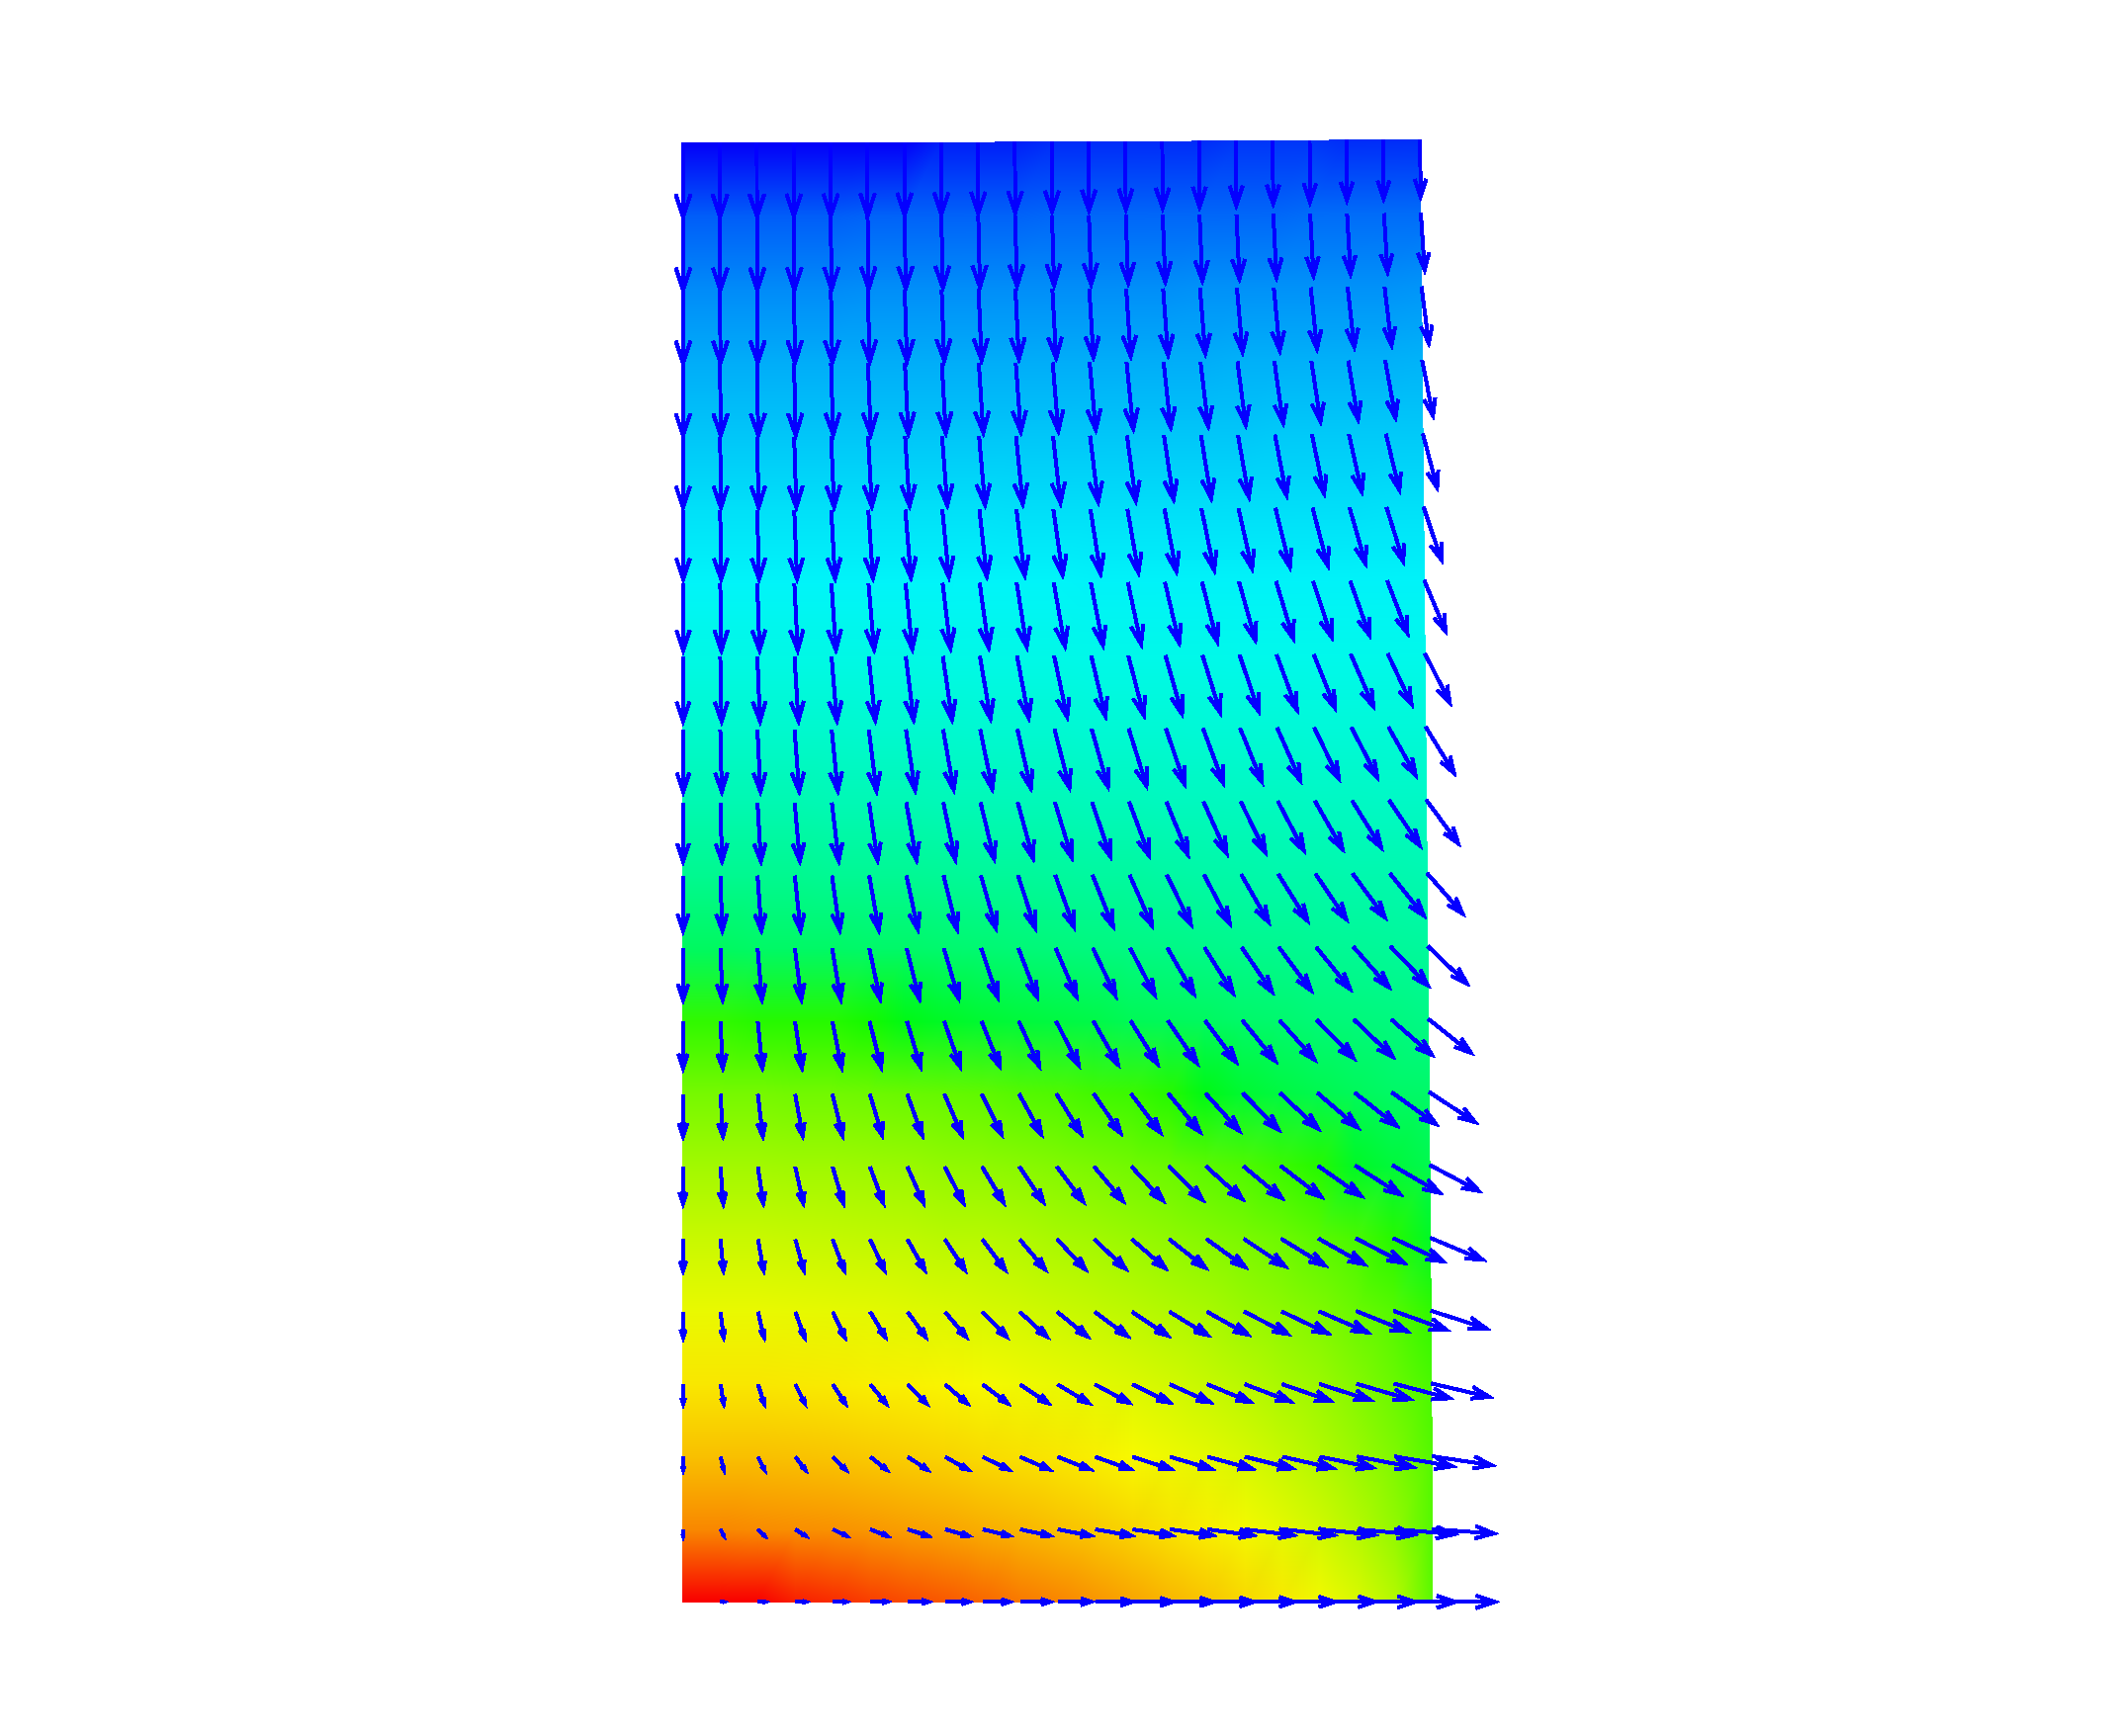
\includegraphics[scale=0.2]{figures/stokes-fluid-t01}}
\subfigure[t=20]{\label{FLOW OUTPUT 10}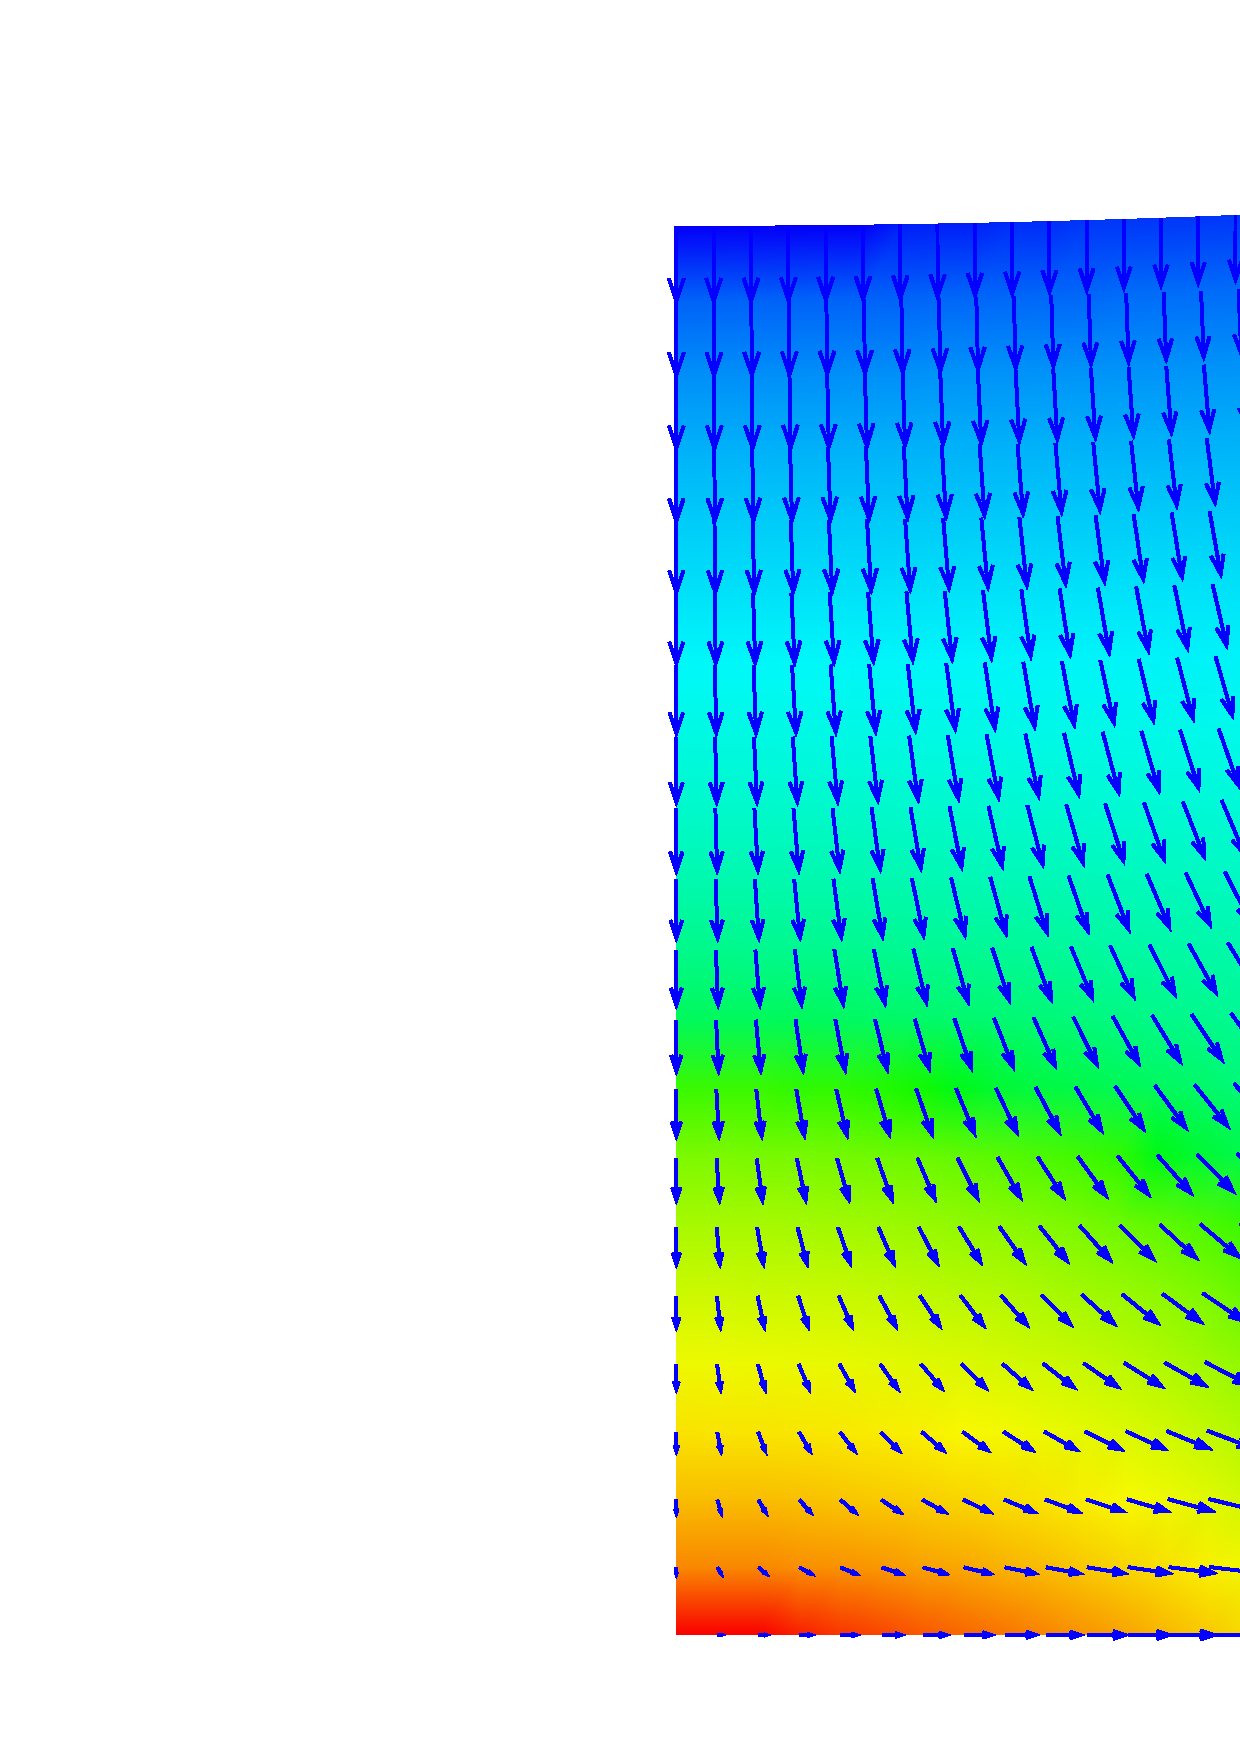
\includegraphics[scale=0.2]{figures/stokes-fluid-t10}}
\subfigure[t=30]{\label{FLOW OUTPUT 20}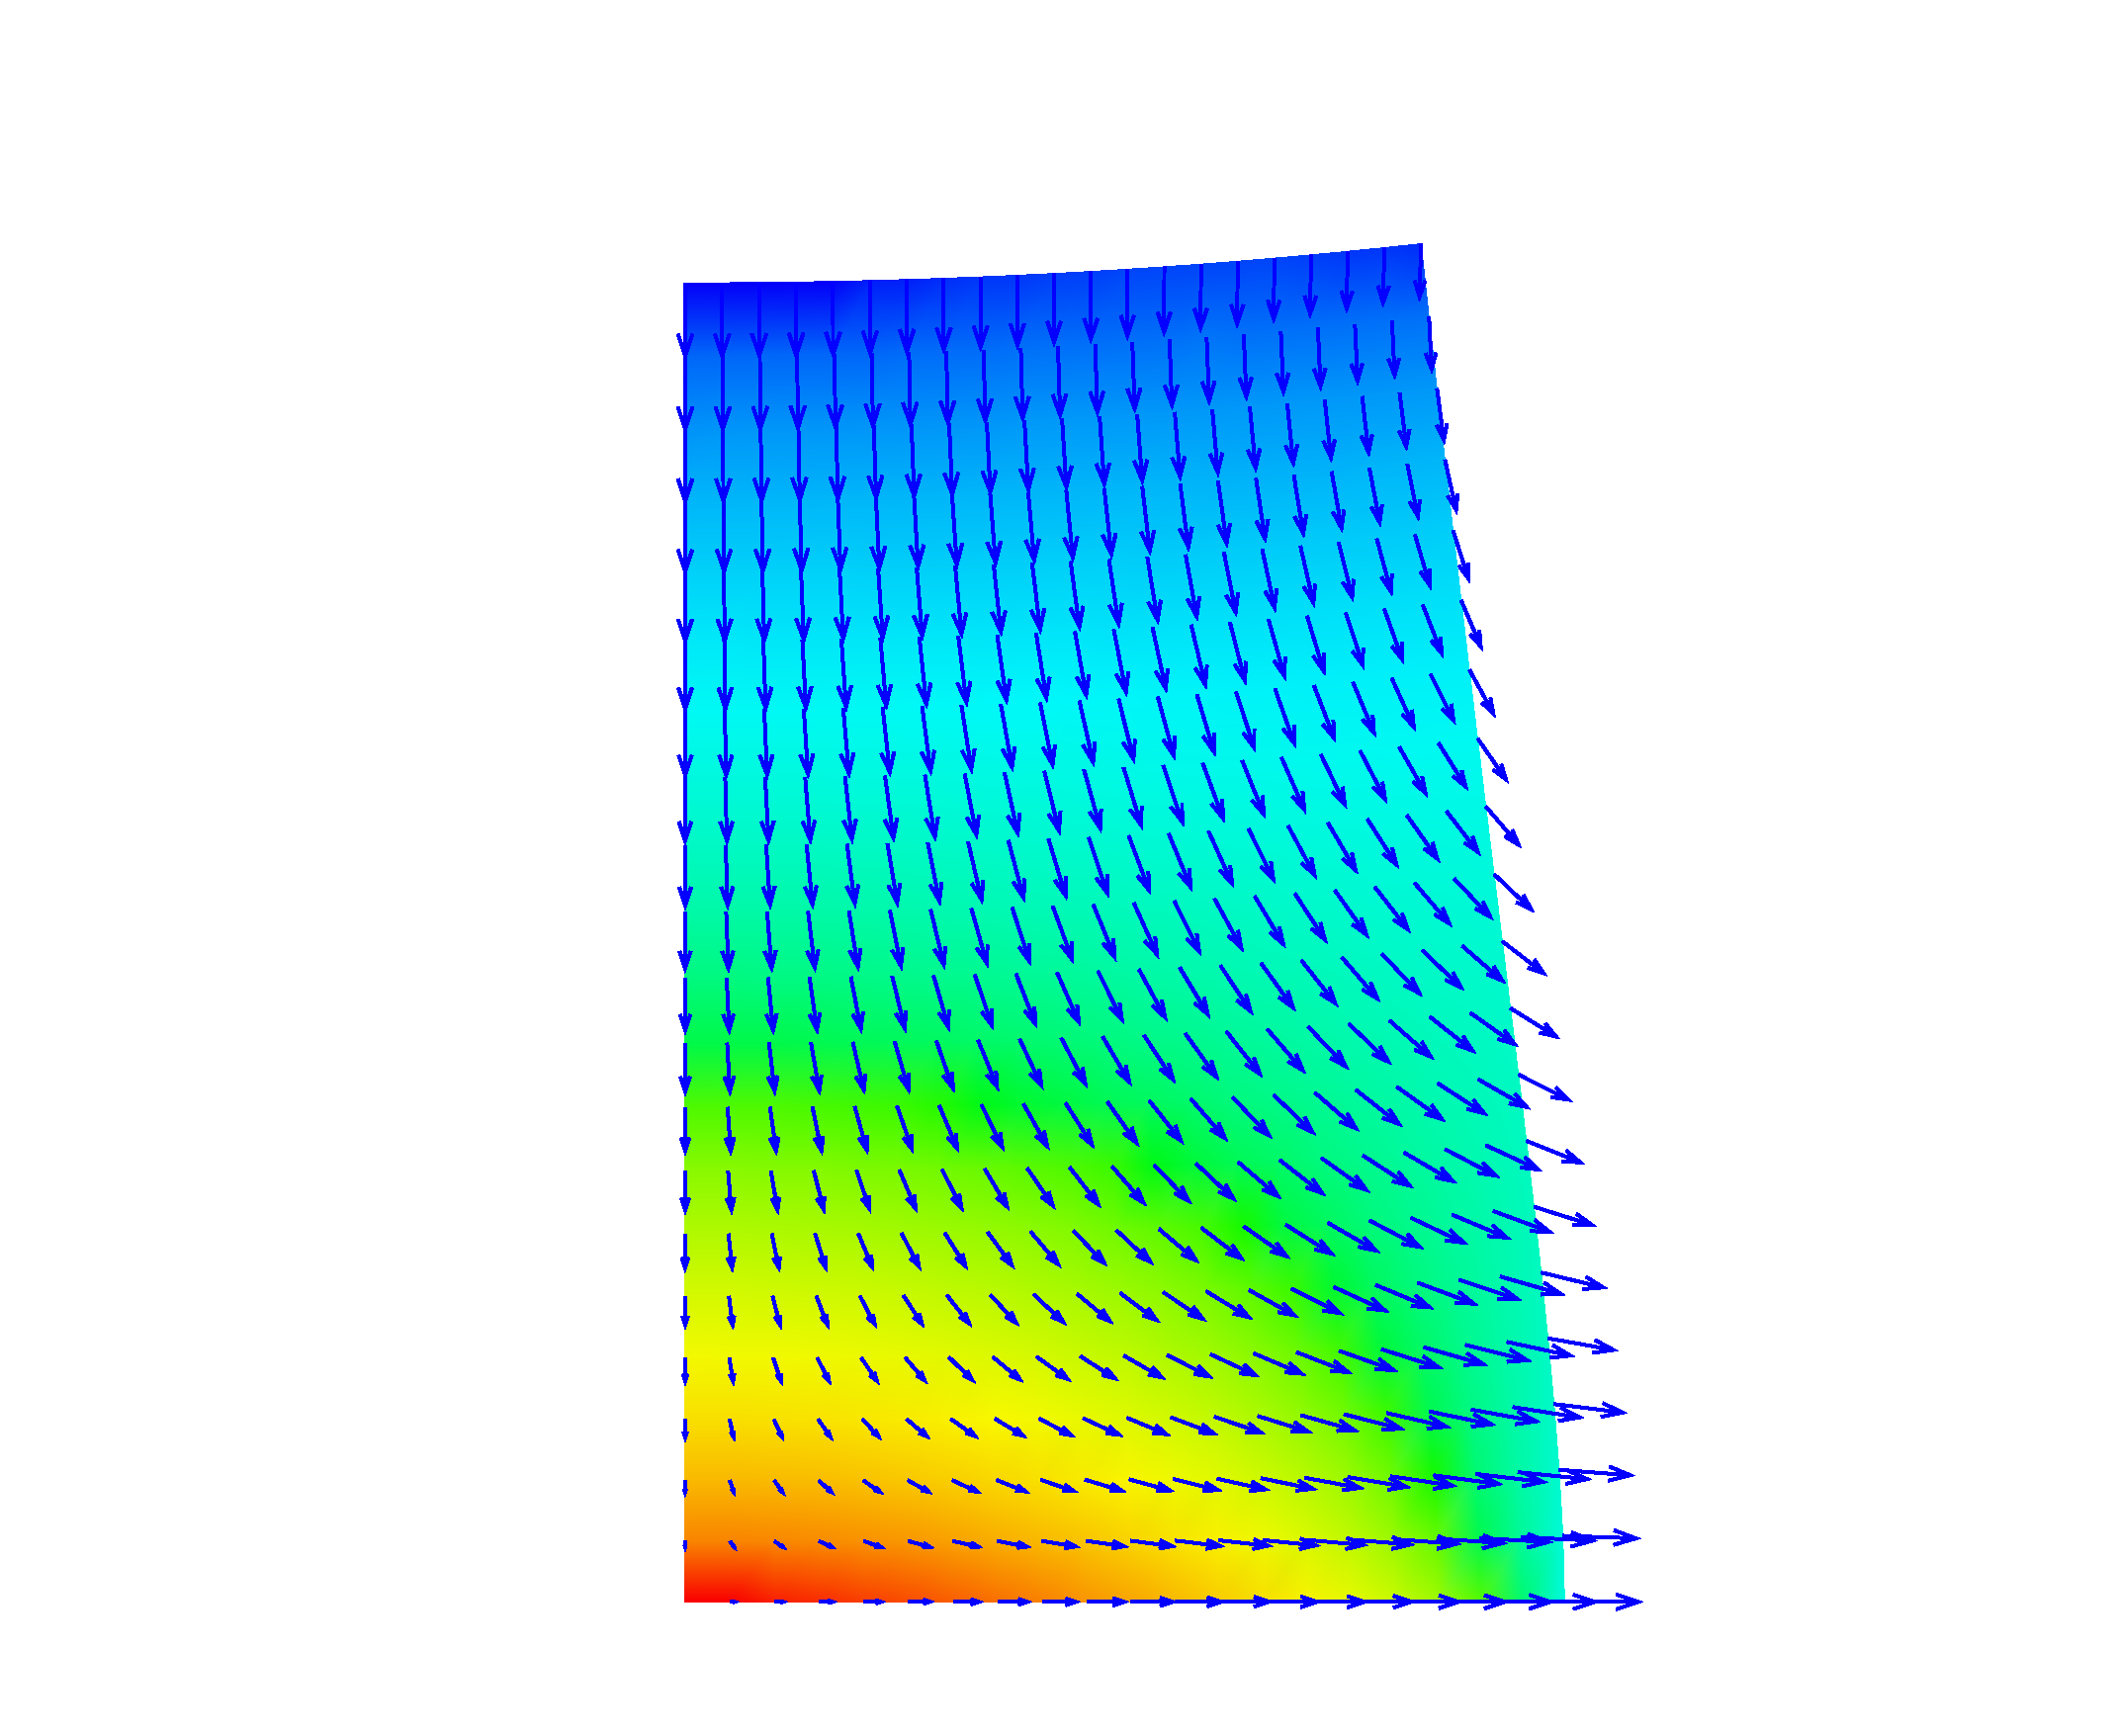
\includegraphics[scale=0.2]{figures/stokes-fluid-t20}}
%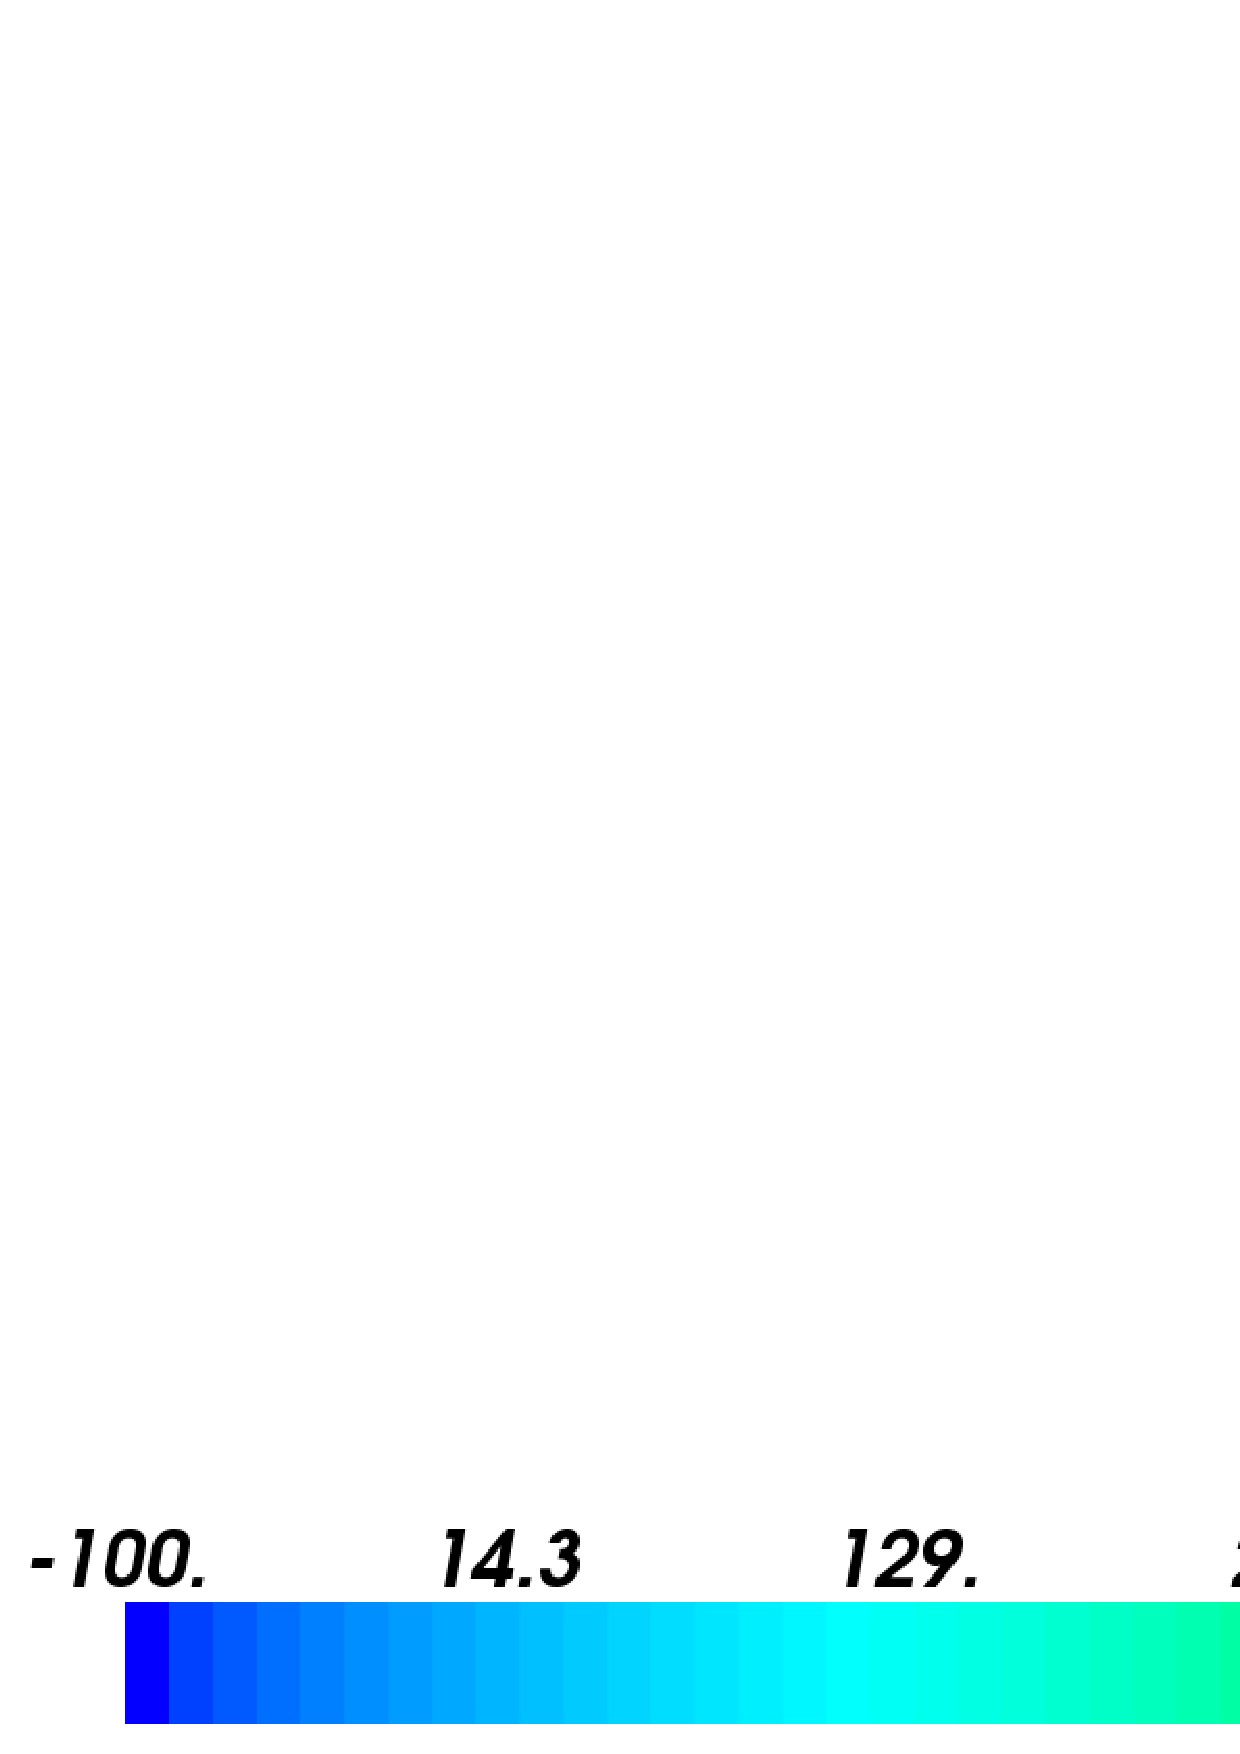
\includegraphics[scale=0.25]{figures/stokes-fluid-colorbar}
\caption{Simulation output for Stokes flow. Fluid body starts off as a rectangular shape, then progresses downwards under the influence of gravity. Color coded distribution represents the scalar values for pressure. Velocity vectors are displayed at each node in the mesh to show the flow field. Computational mesh used was 20$\times$20 elements.}
\label{FLUID OUTPUT1}
\end{figure}
%
\begin{figure}[ht]
\center
\subfigure[t=40]{\label{FLOW OUTPUT 30}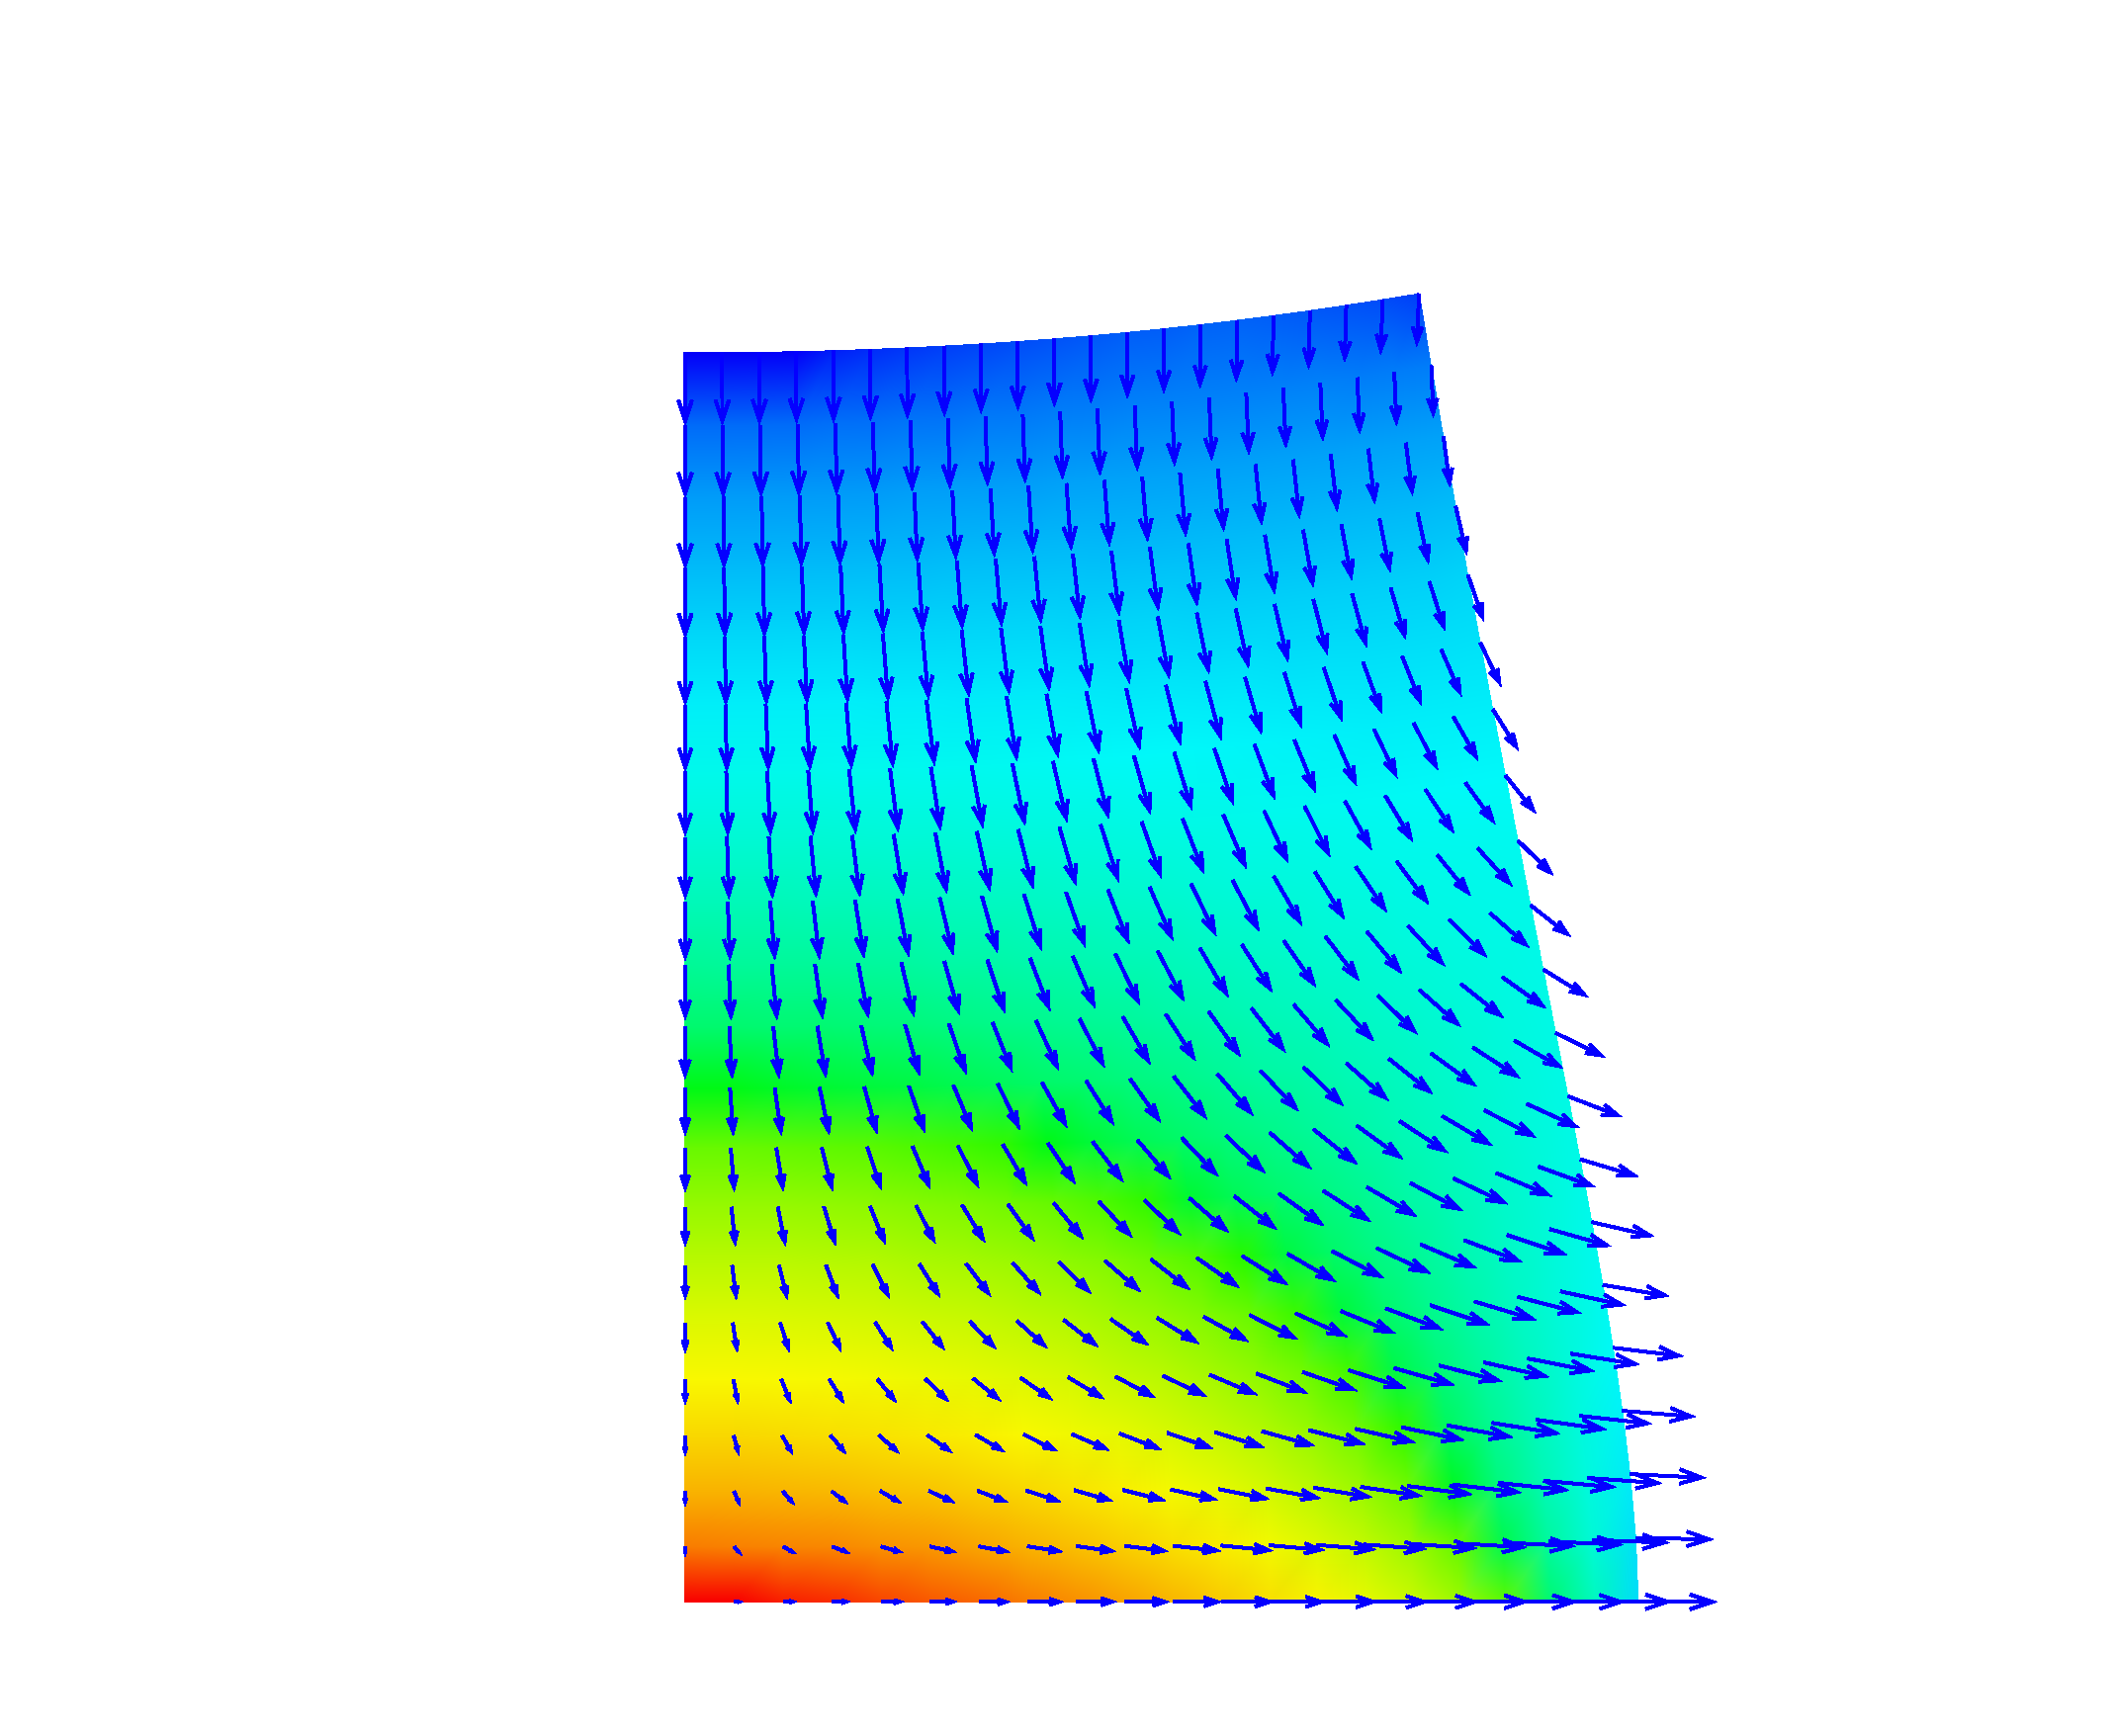
\includegraphics[scale=0.2]{figures/stokes-fluid-t30}}
\subfigure[t=50]{\label{FLOW OUTPUT 40}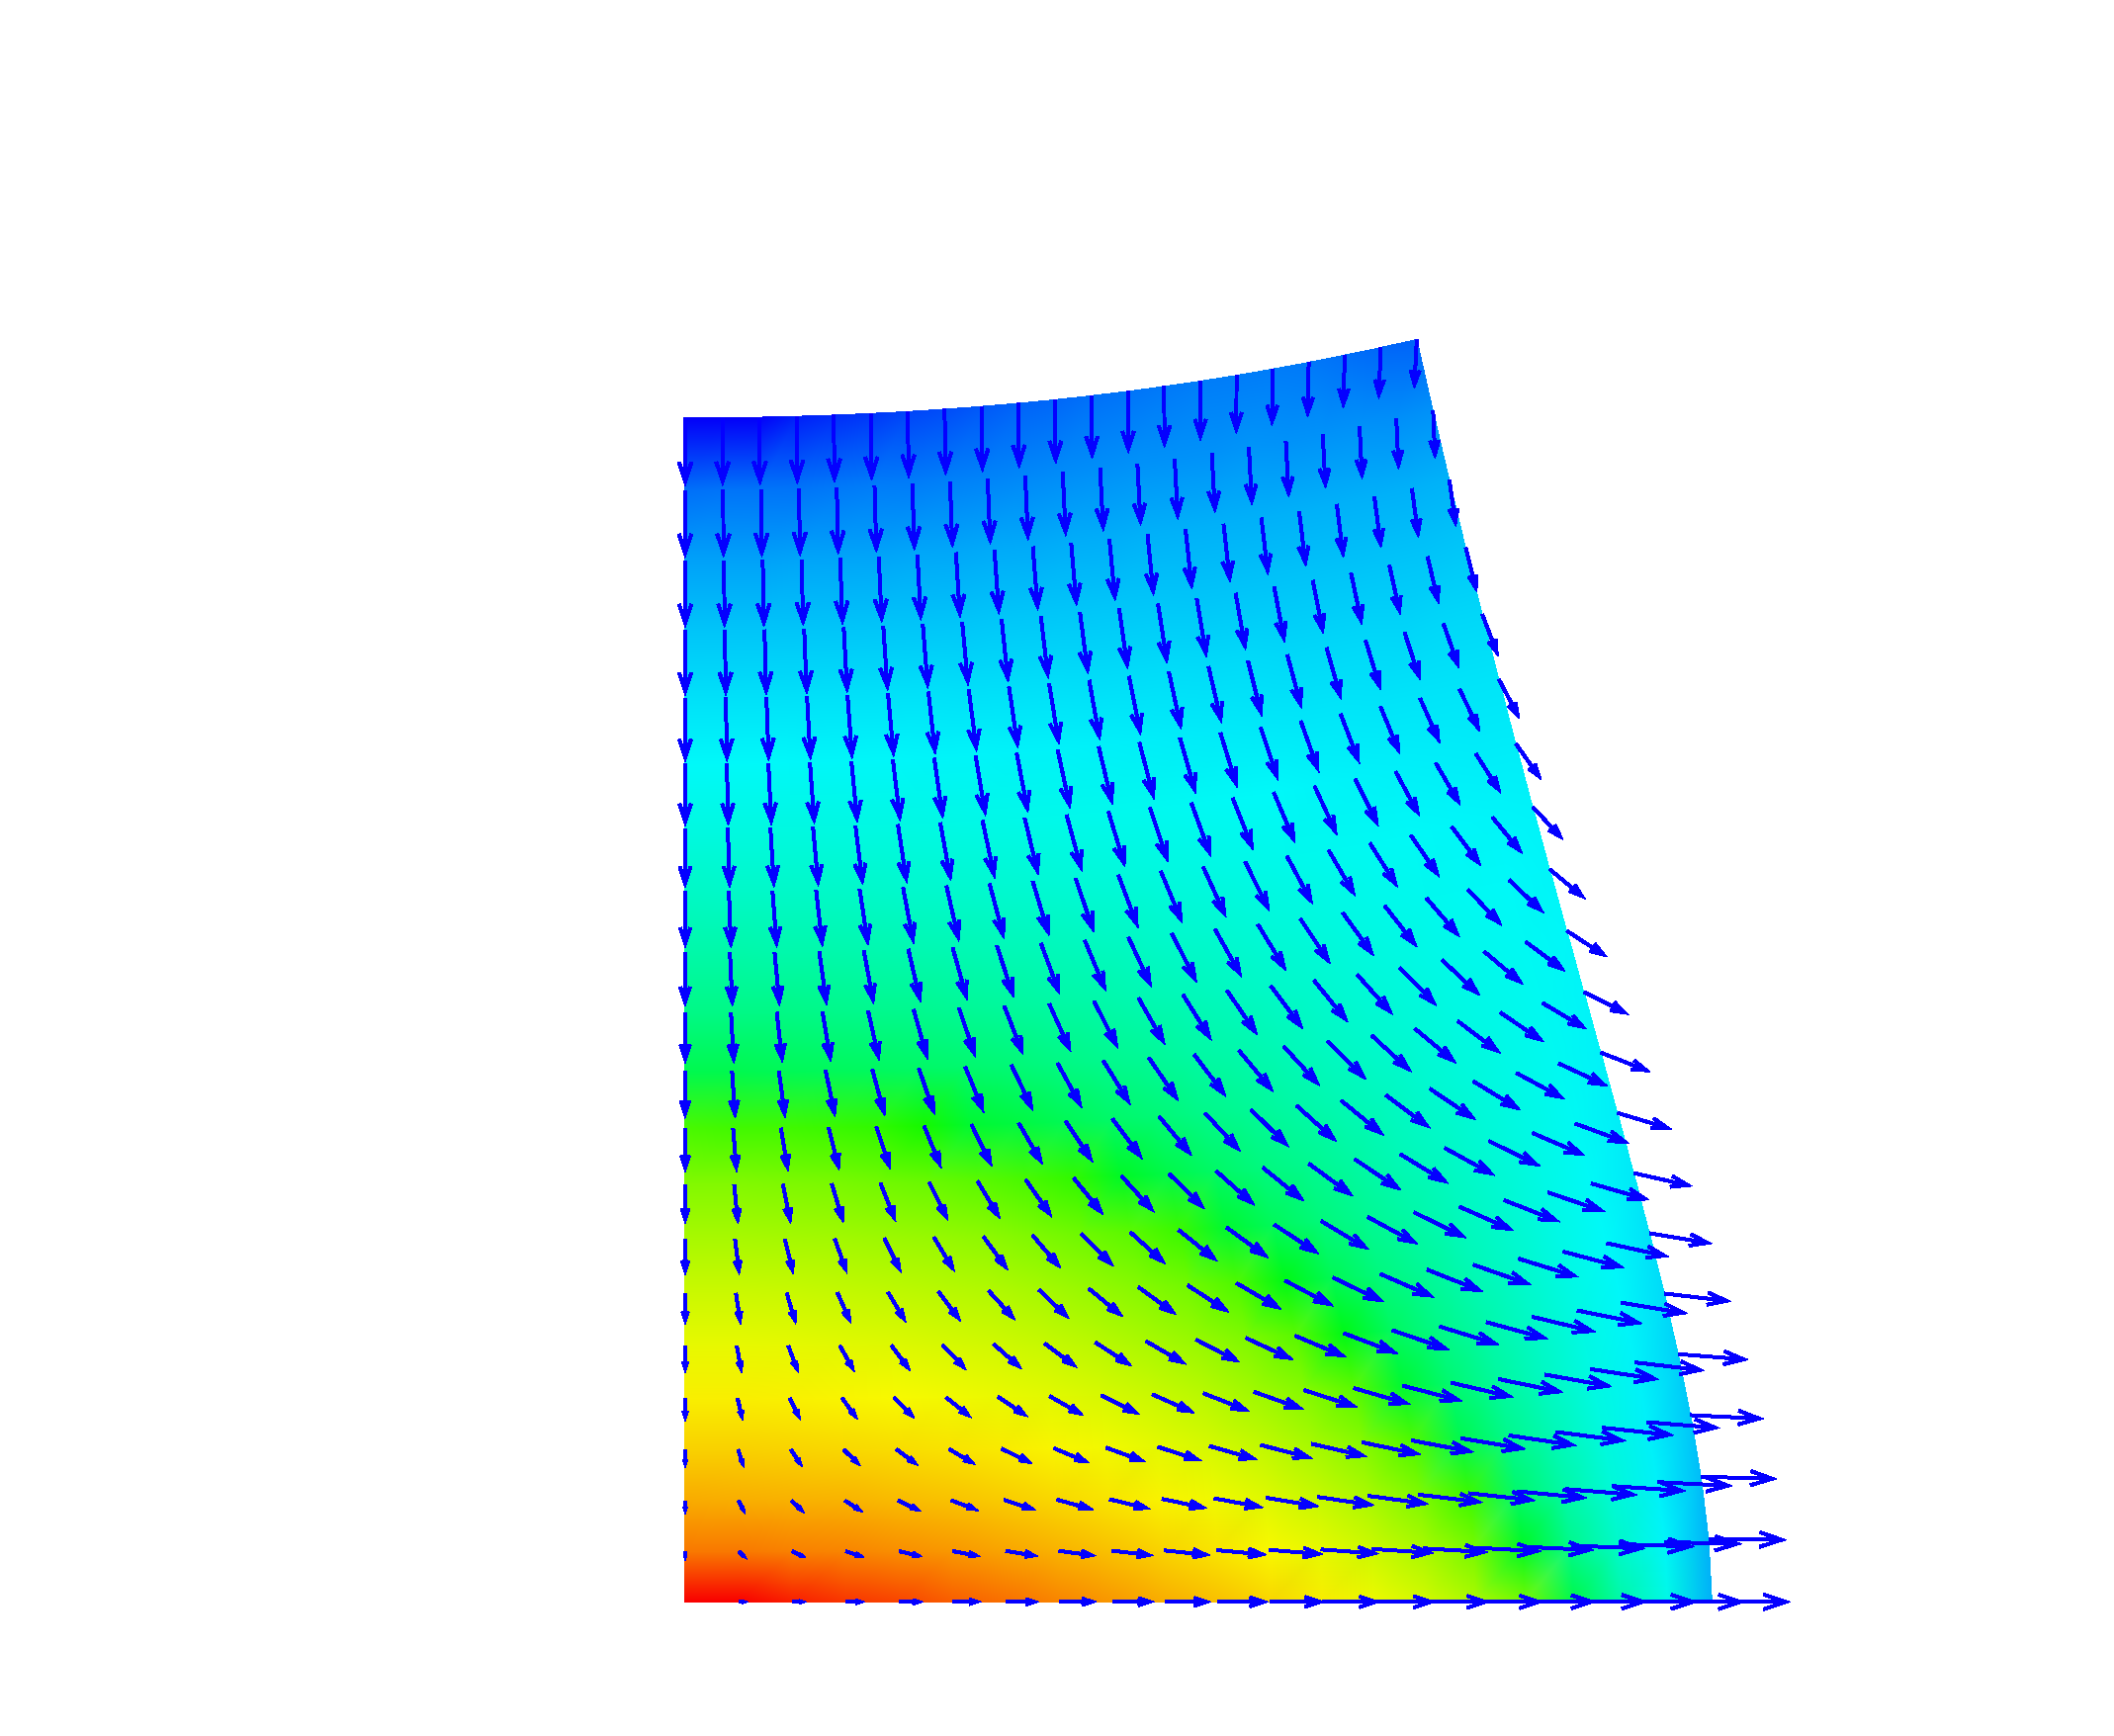
\includegraphics[scale=0.2]{figures/stokes-fluid-t40}}
\subfigure[t=60]{\label{FLOW OUTPUT 50}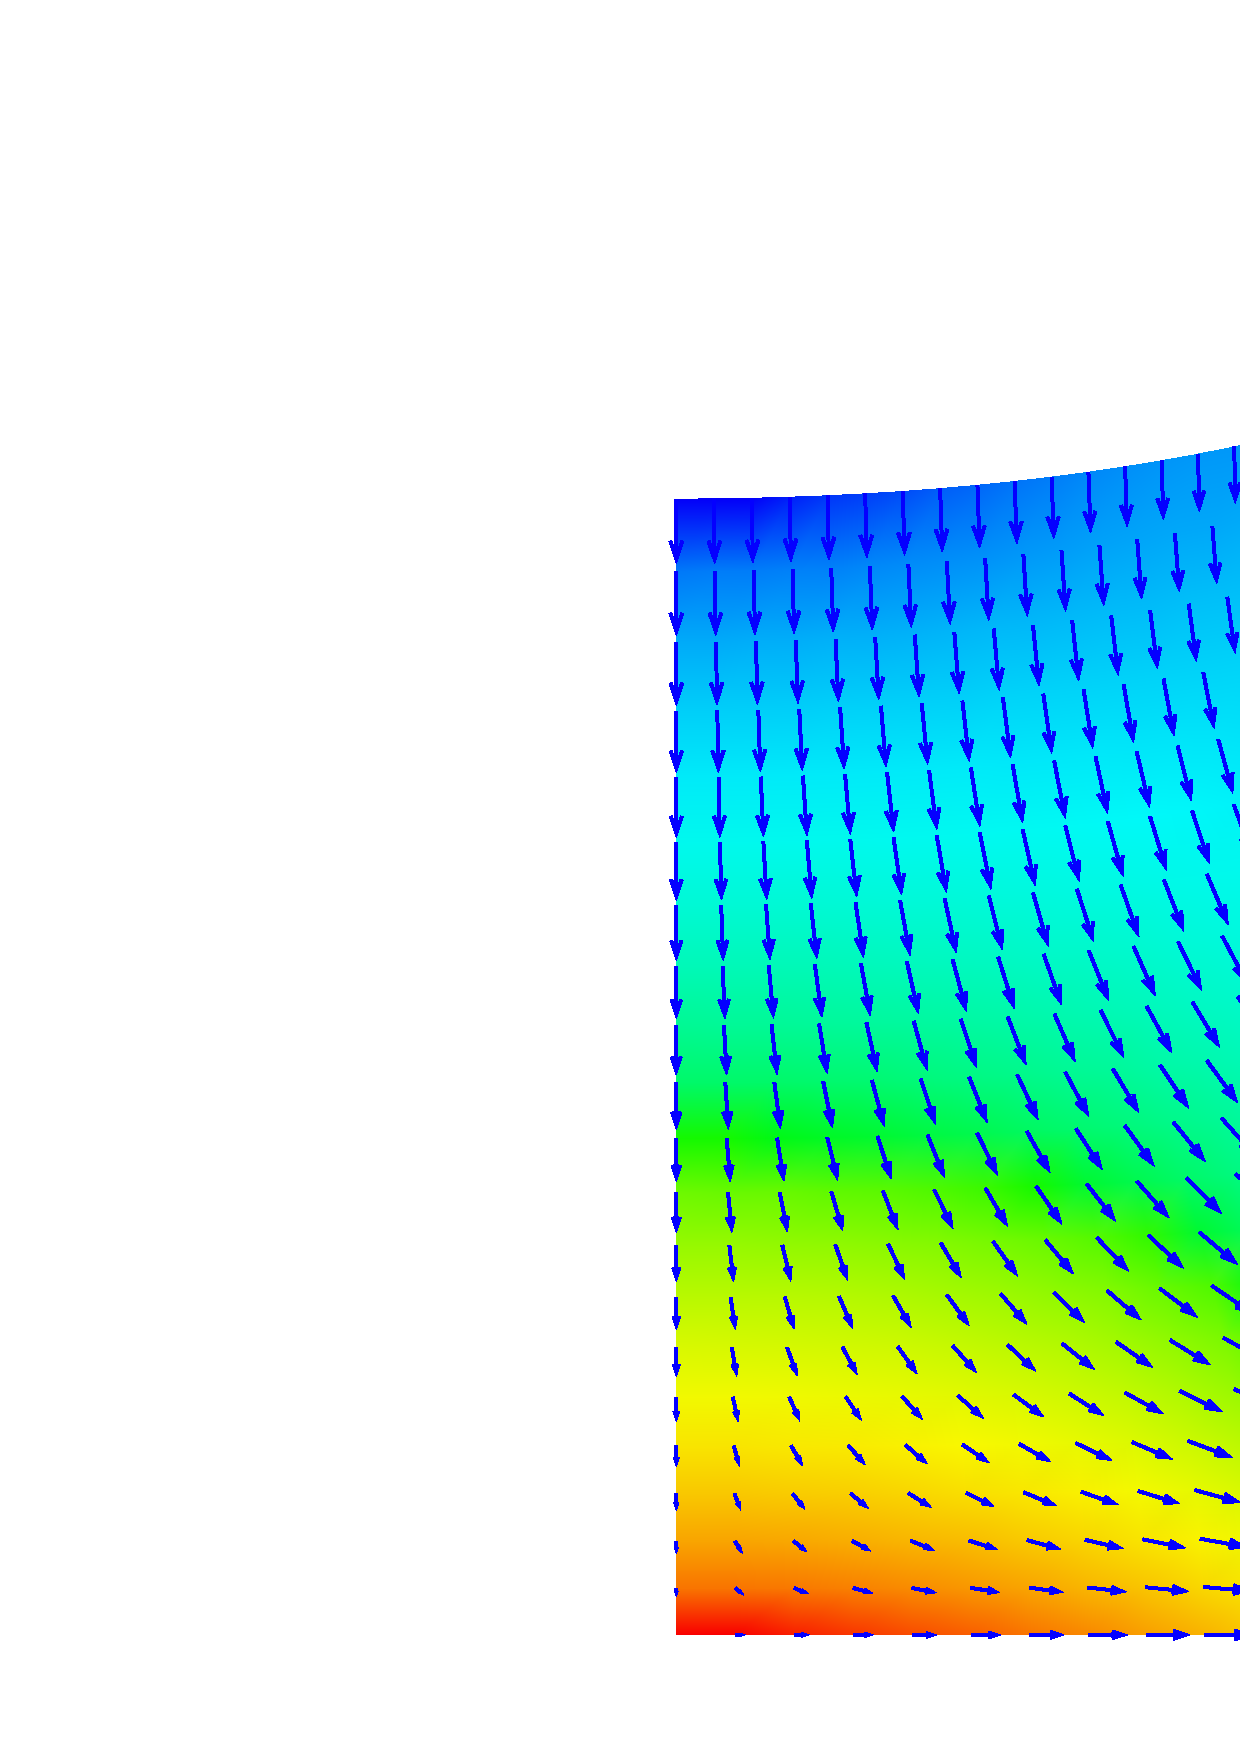
\includegraphics[scale=0.2]{figures/stokes-fluid-t50}}
%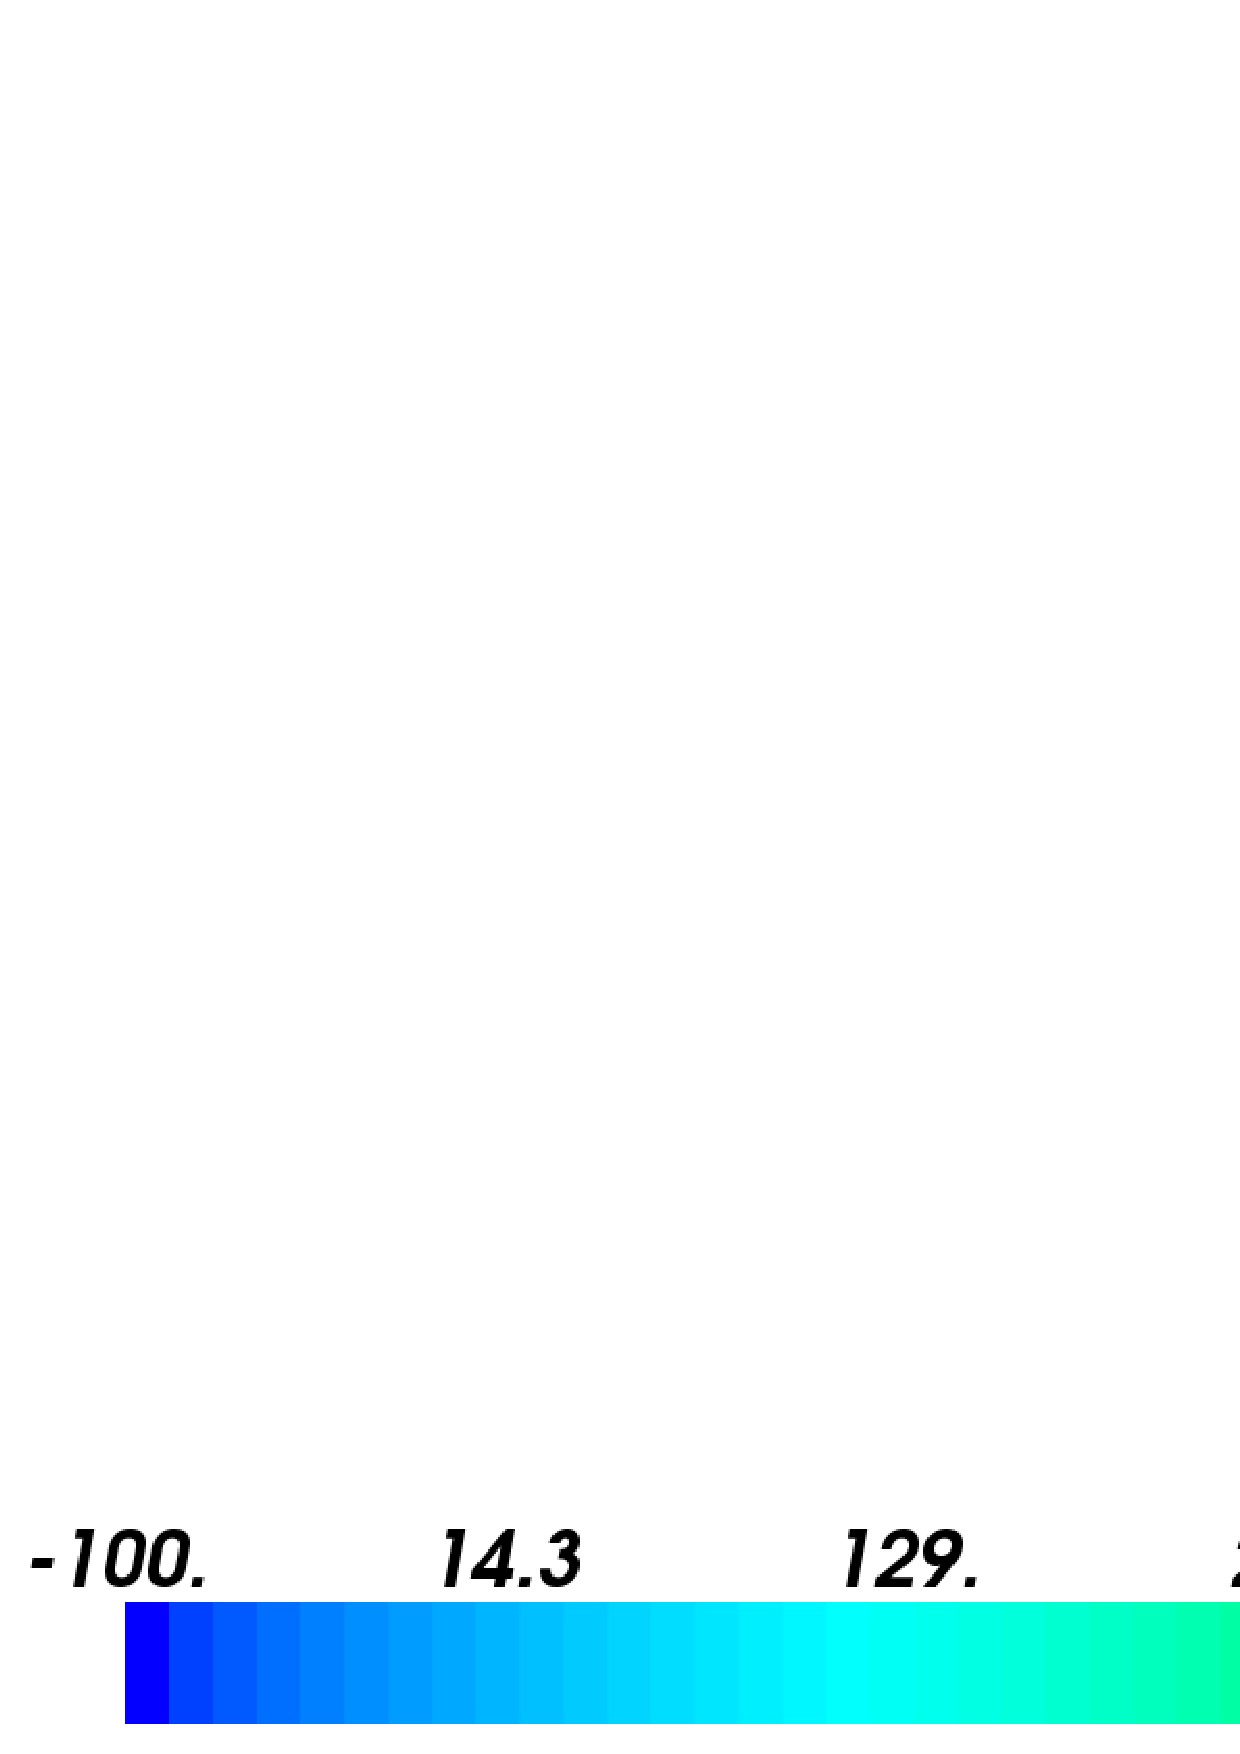
\includegraphics[scale=0.25]{figures/stokes-fluid-colorbar}
\caption{Simulation output for Stokes flow.}
\label{FLUID OUTPUT2}
\end{figure}
%
The view used here to track the fluid is the Lagrangian view, since the mesh moves with the fluid. One of the disadvantages of using the Lagrangian view is that the elements in the mesh become severely distorted after a period of time and introduce solver errors. To get around this limitation the Level Set Method can be used, with the Eulerian point of view for a fixed mesh. 
%The Level Set Method is discussed in Section \ref{LEVELSET CHAP}.
